\documentclass{article}
\usepackage[utf8]{inputenc}
\usepackage{multicol}
\usepackage{listings}
\usepackage{verbatim}
\usepackage{color}
\usepackage{geometry}

\usepackage{float}
\usepackage{amsmath}
\usepackage{hyperref}
\setlength{\belowcaptionskip}{-10pt}
\setlength{\abovecaptionskip}{-30pt}
\floatstyle{boxed} 
\restylefloat{figure}
\usepackage{graphicx}
\definecolor{codegreen}{rgb}{0,0.6,0}
\definecolor{codegray}{rgb}{0.5,0.5,0.5}
\definecolor{codepurple}{rgb}{0.58,0,0.82}
\definecolor{backcolour}{rgb}{0.95,0.95,0.92}

\lstdefinestyle{mystyle}{
	backgroundcolor=\color{backcolour},   
	commentstyle=\color{codegreen},
	keywordstyle=\color{blue},
	numberstyle=\tiny\color{codegray},
	stringstyle=\color{codepurple},
	basicstyle=\footnotesize,
	breakatwhitespace=false,         
	breaklines=true,                 
	captionpos=b,                    
	keepspaces=true,                 
	numbers=left,                    
	numbersep=5pt,                  
	showspaces=false,                
	showstringspaces=false,
	showtabs=false,                  
	tabsize=2
}

\lstset{style=mystyle}
\title{Data Mining\\
		Home work 05\\Q-Q-plots and frequent itemsets}
\author{Aqeel Labash\\ \textbf{Lecturer:} Jaak Vilo}
\date{6 March 2016}

\geometry{
	a4paper,
	total={170mm,257mm},
	left=10mm,
	top=5mm,
}
\begin{document}
	\maketitle
	\section*{First Question}
\textbf{Use the data of child height/weight and study them using qq-plots in a specific age and gender at a time. }\\
Firstly I removed unneeded data and removed the negative values by this code :
\begin{lstlisting}[language=R]
rm(list=ls())
setwd('/home/aqeel/Study/DM/HW05')
ncmp = read.csv('ncmp_1415_final_non_disclosive.csv',header = TRUE)
ncmp$ncmppseudosystemid<-NULL
ncmp$heightzscore<-NULL
ncmp$suppress_imd<-NULL
ncmp$heightpscore<-NULL
ncmp$weightzscore<-NULL
ncmp$weightpscore<-NULL
ncmp$bmizscore<-NULL
ncmp$bmipscore<-NULL
ncmp$suppress_table<-NULL
ncmp$suppress_record_low<-NULL
ncmp$schooltier1localauthority<-NULL
ncmp$suppress_record_high<-NULL
ncmp$suppress_record_high<-NULL
ncmp$pupilschooldistancebanded<-NULL
ncmp$schooltier2localauthority<-NULL
ncmp$schoolgovernmentofficeregion<-NULL
ncmp <- ncmp[ncmp$height>0,]
datasample<-ncmp[sample(nrow(ncmp),5000),]
\end{lstlisting}
After that I tried to get the age with most kids in it by running this code :
\begin{lstlisting}[language=R]
test <-table(ncmp$ageinmonths)
test[test==max(test)]
\end{lstlisting}
Which lead to age 60.6 with 7346 kid.I used the following code to separate male,females and plot height vs weight under age 60.6
\begin{lstlisting}[language=R]
male<- ncmp[ncmp$ageinmonths==60.6&
ncmp$genderdescription=="Male",]
female<-ncmp[ncmp$ageinmonths==60.6&
ncmp$genderdescription=="Female",]

png ('male.png',width = 1200,height = 830)
qqplot(male$height,male$weight)
dev.off()
png ('female.png',width = 1200,height = 830)
qqplot(female$height,female$weight)
dev.off()
\end{lstlisting}
\begin{figure}[H]
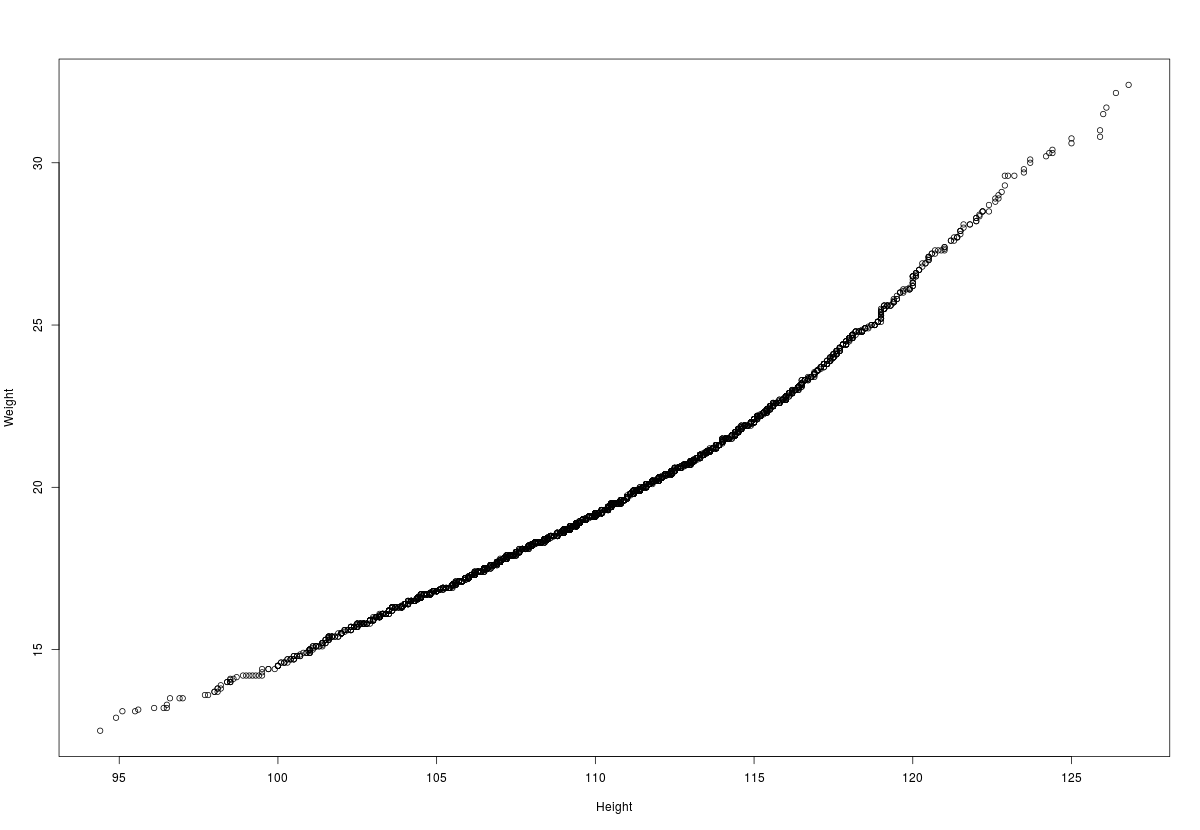
\includegraphics[scale=0.4]{male.png}
\caption{Weight vs height for male kids at age 60.6}
\end{figure}
From figure 1 can notice that height and weight are highly correlated.
\begin{figure}[H]
	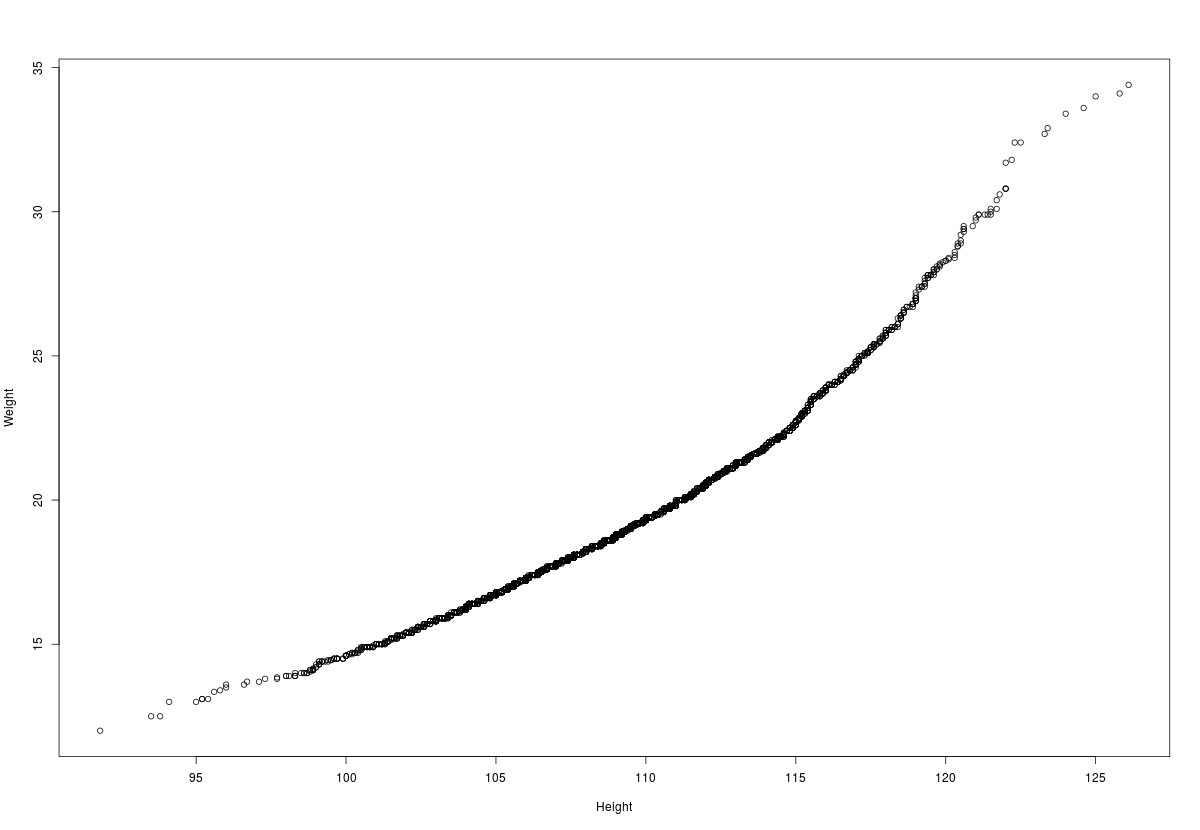
\includegraphics[scale=0.4]{female.png}
	\caption{Weight vs height for male kids at age 60.6}
\end{figure}
In figure 2 we can notice that they are also correlated but if we compare figure 1 with figure 2 we can notice that the weight growth with height slightly higher.\\
\textbf{Compare heights of underweight and very overweight children }\\
To do the comparison I used the following code : 
\begin{lstlisting}[language=R]
underoverweights<- ncmp[ncmp$bmipopulationcategory =='very overweight' | ncmp$bmipopulationcategory=='underweight' ,]
png('undervsover.png',width=1200,height = 830)
ggplot(data = underoverweights, mapping = aes(x=bmipopulationcategory,y=height))+geom_point()
dev.off()
\end{lstlisting}
\begin{figure}[H]
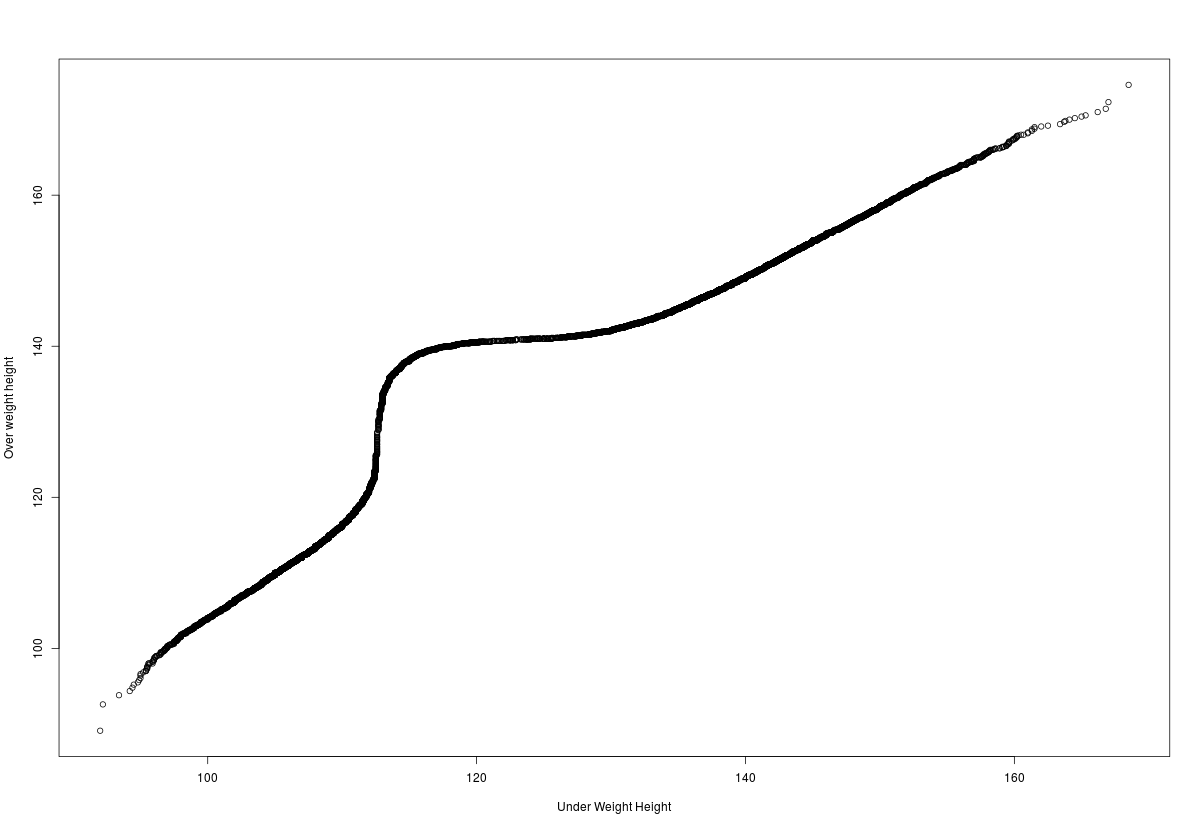
\includegraphics[scale = 0.4]{undervsover.png}
\caption{Comparison under weight vs very over weight height }
\end{figure}
From figure 3 we can see that over weight kids and under weight kids have almost same distribution but I would say that there is high percentage of under weight kids with heights around 110.The following code is what I used to accomplish it:
\begin{lstlisting}[language=R]

underweight<- ncmp[ncmp$bmipopulationcategory =='very overweight' ,]
overweight<-ncmp[ncmp$bmipopulationcategory=='underweight',]
png('undervsover.png',width=1200,height = 830)
qqplot(underweight$height,overweight$height,xlab = 'Under Weight Height',ylab = 'Over weight height')
dev.off()
\end{lstlisting}
\textbf{Compare one of the attributes (height, weight, BMI) between boys and girls (select either younger or older age group) to each other. }\\
For this task I selected the younger age group. and used the following code :
\begin{lstlisting}[language=R]
agelimits<-c(49.1,70.0,120.8,141.4)
maleage1 <-ncmp[ncmp$ageinmonths>agelimits[1] & ncmp$ageinmonths<agelimits[2]&
ncmp$genderdescription=="Male",]

femaleage2 <-ncmp[ncmp$ageinmonths>agelimits[1] & ncmp$ageinmonths<agelimits[2]&
ncmp$genderdescription=="Female",]
png('malevsfemale.png',width=1200,height = 830)
qqplot(maleage1$height,femaleage2$height)
dev.off()
\end{lstlisting}
\begin{figure}[H]
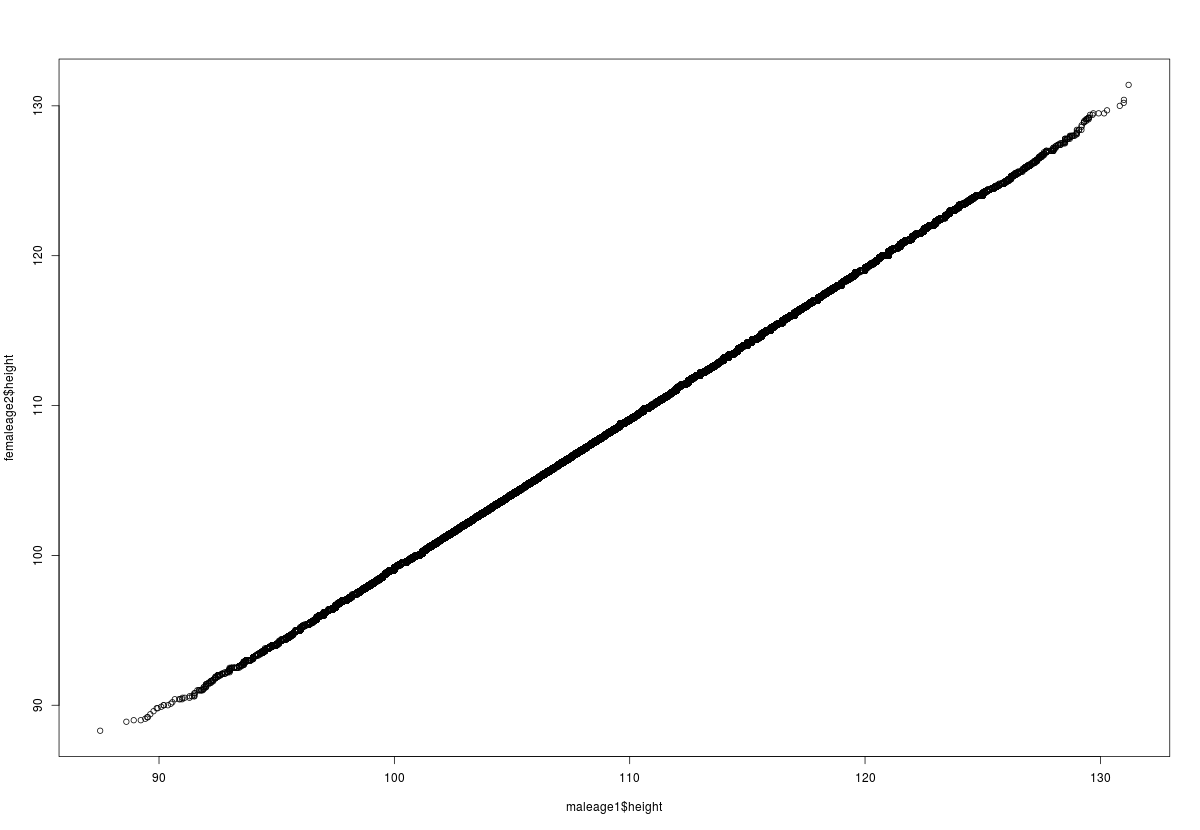
\includegraphics[scale=0.4]{malevsfemale.png}
\caption{Q-Q plot for heights male vs female}
\end{figure}
From previous plot we can see that it's almost linear plot which mean at this age almost female and male have the same height.In other worlds sex doesn't affect the height at this age.
	\section*{Second Question}
For this question I used the groups I created for the first question with same age 60.6 and used the following code for the plots:
\begin{lstlisting}[language=R]
png('malebmi.png',width = 1200,height = 830)
qqplot(male$height,male$bmi)
dev.off()
png('femalebmi.png',width = 1200,height = 830)
qqplot(female$height,female$bmi)
dev.off()
\end{lstlisting}
\begin{figure}[H]
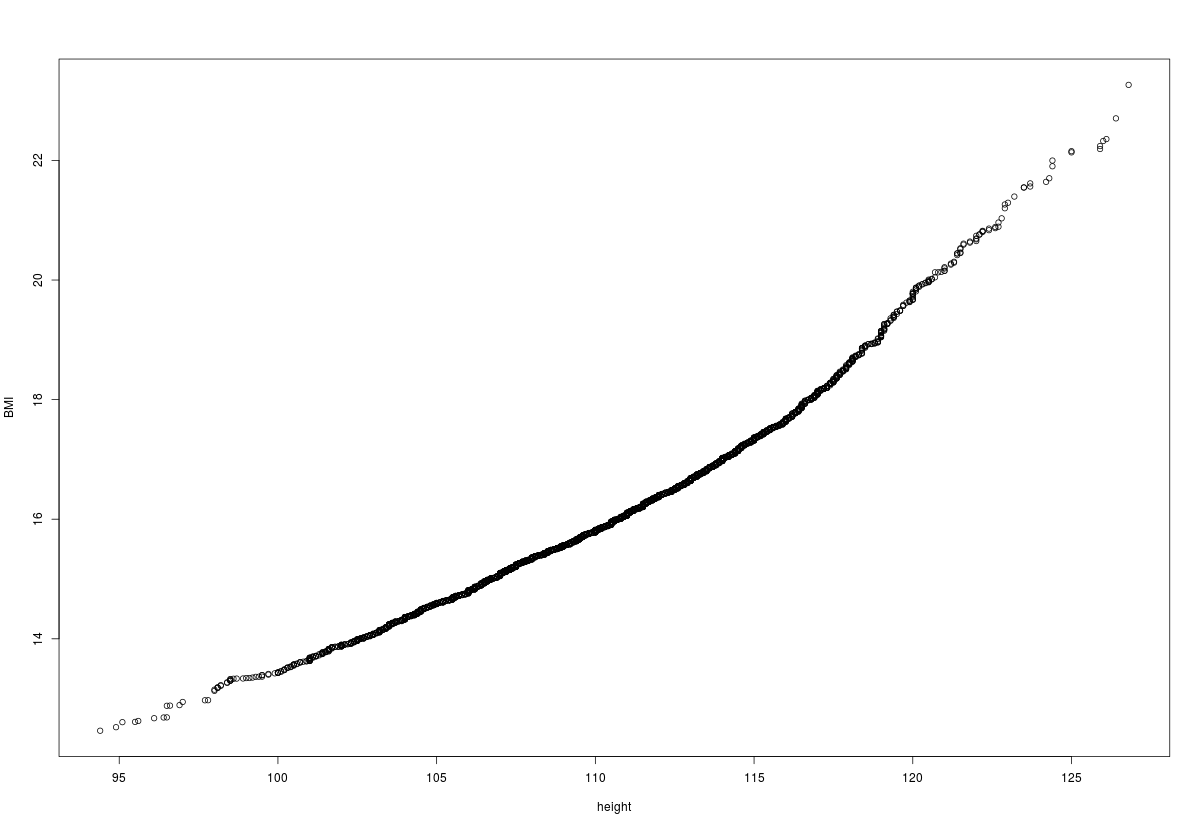
\includegraphics[scale=0.4]{malebmi.png}
\caption{Male age =60.6 , height vs BMI}
\end{figure}
Comparing figure 5 with figure 6 we can notice that females has more BMI than males in the same group of height.
\begin{figure}[H]
	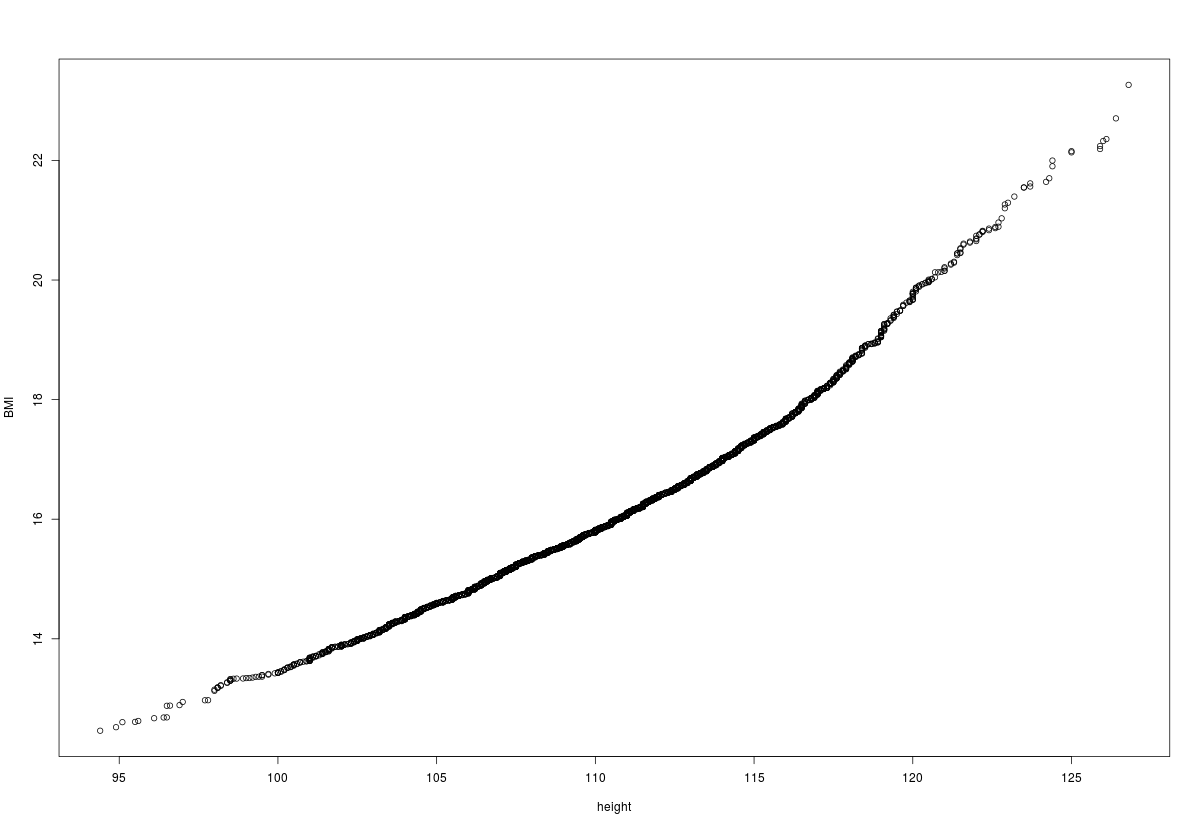
\includegraphics[scale=0.4]{malebmi.png}
	\caption{Female age =60.6 , height vs BMI}
\end{figure}
	\section*{Third Question}
	For this task I took the male gender from 60.6 to 80 (about 15000 kid) for over weight children. I used the following code :
	\begin{lstlisting}[language=R]
########Third Question #############
overweight<-ncmp[ncmp$bmipopulationcategory=='overweight'&ncmp$genderdescription=='Male' &ncmp$ageinmonths>60.6 &
ncmp$ageinmonths<80,]
png('QQvsdest',width = 1200,height = 830)
qqnorm(overweight$height);qqline(overweight$height,col=2);
dev.off()
	\end{lstlisting}
\begin{figure}[H]
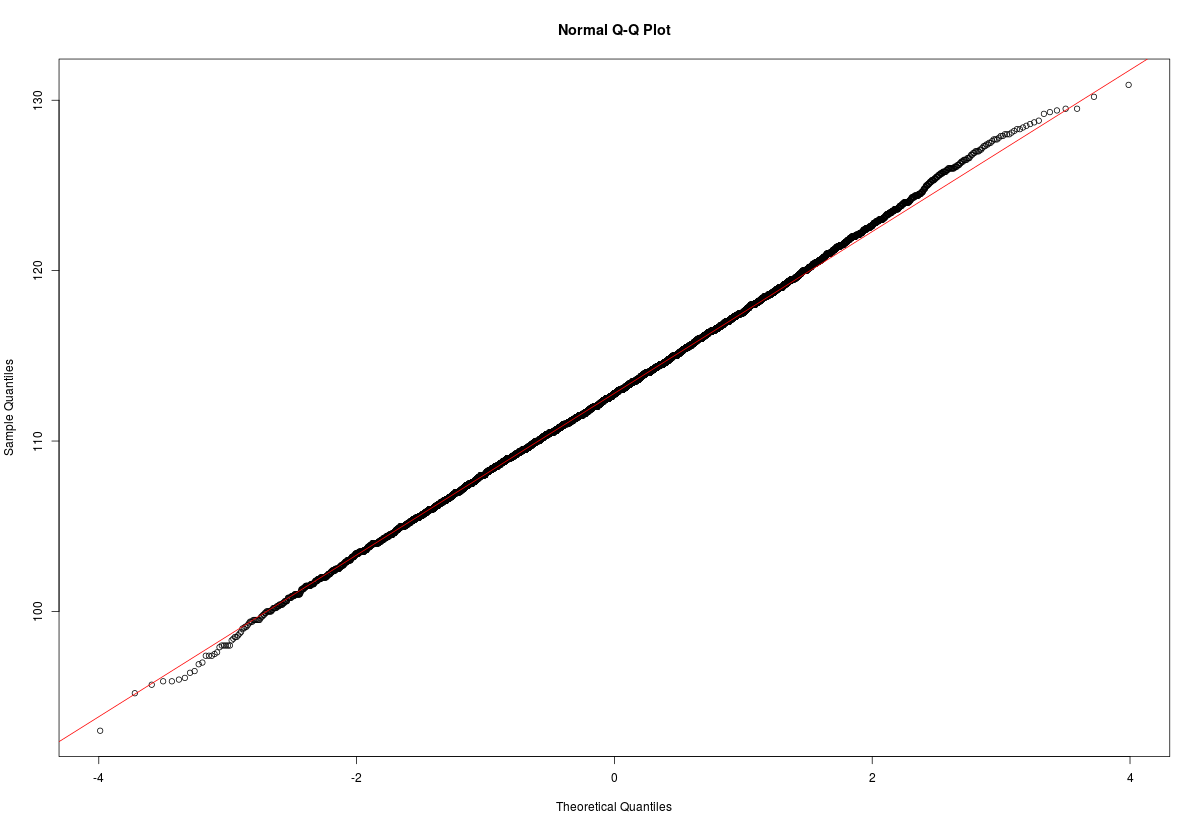
\includegraphics[scale=0.4]{QQvsdest.png}
\caption{Overweight children height vs Theoretical normal distribution}
\end{figure}
Although figure 7 shows that the height almost identical to normal distribution but when we take all the points of overweighted children we would notice a difference.
	\section*{Fourth Question}
\textbf{Note:}I believe the question changed (it was with support more than 3 then become more than 0.3) which is the same in this question (3/8 = 0.375 , 2/8 = 0.25).\\
For this question I used python \\ \textbf{Note: } you need to generalize the last step to get all the combination we want.Here is the code :
\begin{lstlisting}[language=Python]

# coding: utf-8

# In[95]:

import itertools


# In[96]:

main =[]
main.append(sorted(['B','C', 'A' ,'F', 'H']))
main.append(sorted(['F', 'E', 'C', 'H']))
main.append(sorted(['E' ,'D', 'B']))
main.append(sorted(['A', 'C' ,'H', 'F']))
main.append(sorted(['E', 'F' ,'A']))
main.append(sorted(['D', 'H' ,'B']))
main.append(sorted(['E', 'C' ,'F', 'B', 'D']))
main.append(sorted(['A', 'H' ,'C', 'E']))
main.append(sorted(['G', 'A', 'E']))
main.append(sorted(['B', 'H', 'E']))


# In[97]:

lst={}
def addelement(element):
if element not in lst.keys():
lst[element]=1
else:
lst[element]+=1


# In[98]:

for i in main:
for j in i:
addelement(j)


# In[99]:

print len(lst.keys())
for key in lst.keys():
print key,lst[key]
if lst[key]<3:
lst.pop(key,None)
print '------ after cleaning--------'
for key in lst.keys():
print key,lst[key]
print len(lst.keys())


# In[148]:

lst2items={}
def addelement2(el):
el = ''.join(map(str.strip,el))
if el not in lst2items.keys():
lst2items[el]=1
else:
lst2items[el]+=1


# In[149]:

def checkcontain(myelements,thelist):
for i in myelements:
if i.strip() not in thelist:
return False
return True


# In[150]:

newcomb = itertools.combinations(lst.keys(), 3)

for i in newcomb:
for j in main:
if checkcontain(i,j):
addelement2(i)


# In[151]:

for key in lst2items.keys():
print key,lst2items[key]
if lst2items[key]<3:
lst2items.pop(key,None)
print '------ after cleaning--------'
for key in lst2items.keys():
print key,lst2items[key]
\end{lstlisting}
You can find a copy on git hub here \href{https://github.com/aqeel13932/DM}{DM} in Home work 05 folder.\\
I started with one element :
A 5
C 5
B 5
E 7
D 3
F 5
H 6\\
Then for 2 elements :
BD 3
BE 3
AC 3
AE 3
EH 3
AF 3
AH 3
EF 3
BH 3
CF 4
CE 3
CH 4
FH 3\\
Then for 3 elements:
ACH 3
CFH 3\\
And there is no 4 elements with support 3 or more.
	\section*{Fifth Question}
For this question I put all the information in Calc sheet and fulled it with the results I got from 4th question. Here is the heat map:
\begin{figure}[H]
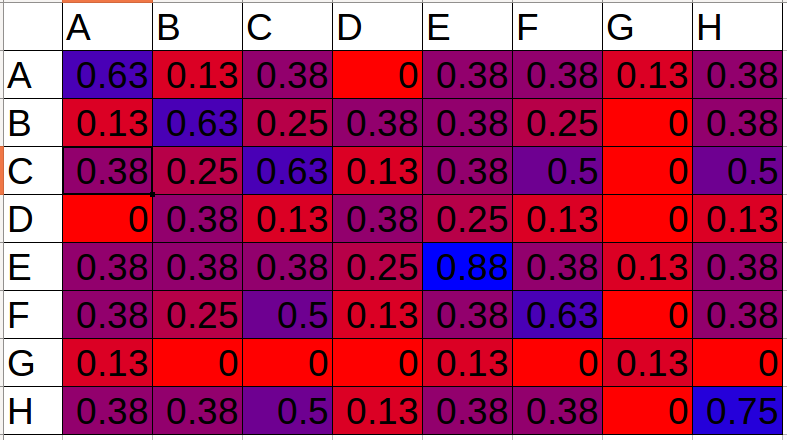
\includegraphics[scale=0.6]{5q.png}
\caption{Heatmap for support}
\end{figure}
To calculate the confidence I actually used a trick :) .In figure 9 you can see the table that I depended on to calculate both (support \& confidence).
\begin{figure}[H]
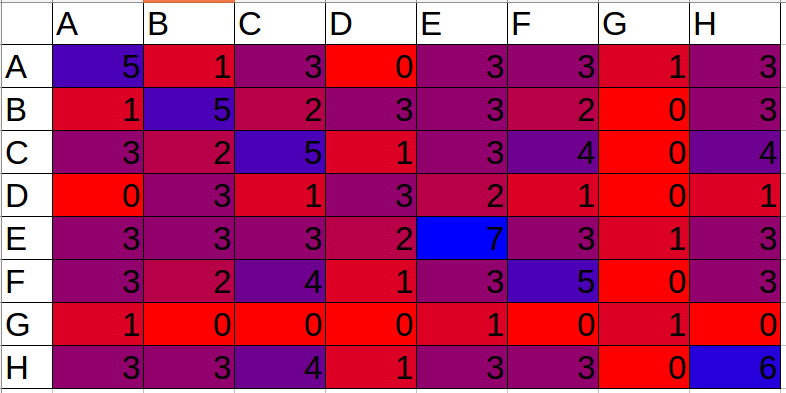
\includegraphics[scale=0.6]{5q3.png}
\caption{Table shows how many two items occurred}
\end{figure}
We can notice that if we divide each cell on 8 (number of transaction) we get the support and if we divide each row on the diagonal element we get the confidence.\\
Here is the confidence table :
\begin{figure}[H]
	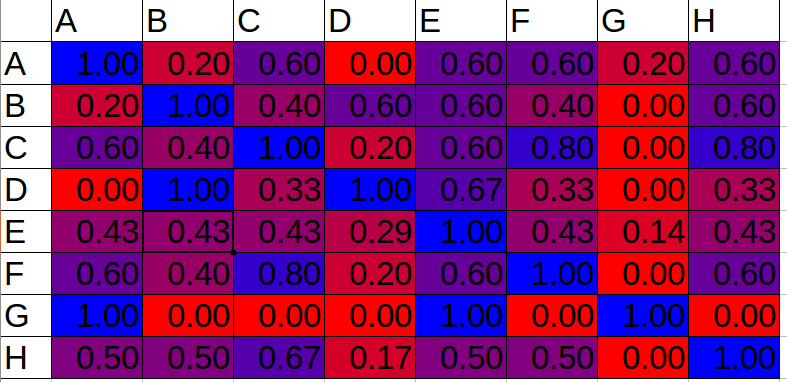
\includegraphics[scale=0.6]{5q2.png}
\caption{Confidence table}
\end{figure}
\end{document}